% Results Bar Chart
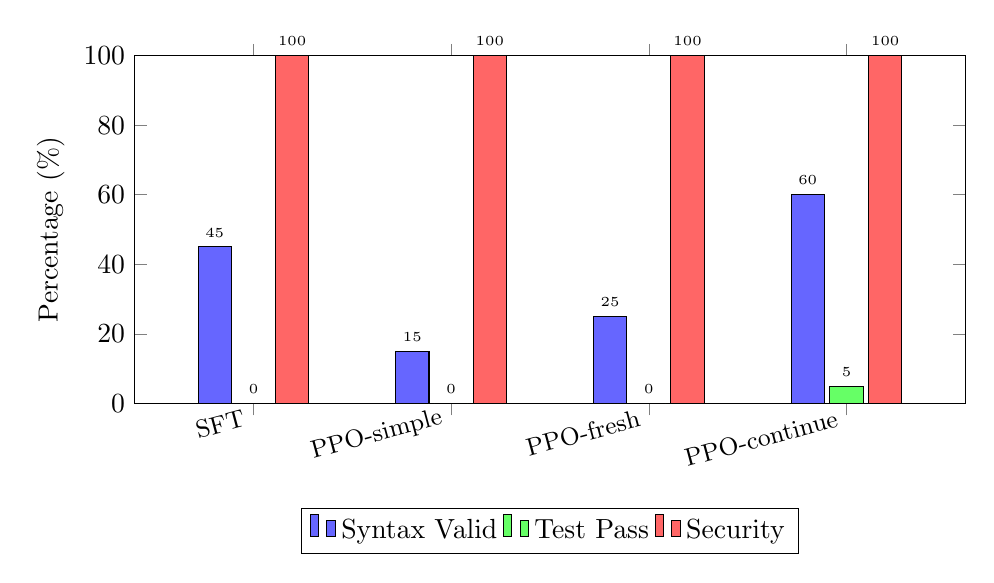
\begin{tikzpicture}
\begin{axis}[
    ybar,
    bar width=12pt,
    width=\columnwidth,
    height=6cm,
    ylabel={Percentage (\%)},
    symbolic x coords={SFT, PPO-simple, PPO-fresh, PPO-continue},
    xtick=data,
    x tick label style={rotate=15, anchor=east, font=\small},
    ymin=0,
    ymax=100,
    legend style={at={(0.5,-0.3)}, anchor=north, legend columns=3},
    nodes near coords,
    nodes near coords align={vertical},
    every node near coord/.append style={font=\tiny},
    enlarge x limits=0.2,
]

% Syntax Pass Rate
\addplot[fill=blue!60] coordinates {
    (SFT, 45)
    (PPO-simple, 15)
    (PPO-fresh, 25)
    (PPO-continue, 60)
};

% Test Pass Rate
\addplot[fill=green!60] coordinates {
    (SFT, 0)
    (PPO-simple, 0)
    (PPO-fresh, 0)
    (PPO-continue, 5)
};

% Security Compliance
\addplot[fill=red!60] coordinates {
    (SFT, 100)
    (PPO-simple, 100)
    (PPO-fresh, 100)
    (PPO-continue, 100)
};

\legend{Syntax Valid, Test Pass, Security}
\end{axis}
\end{tikzpicture}
